\documentclass[11pt]{article}
\usepackage[T1]{fontenc}
\usepackage[utf8]{inputenc}
\usepackage{lmodern}
\usepackage[margin=1in]{geometry}
\usepackage{amsmath,amssymb,amsthm,mathtools}
\usepackage{enumitem,microtype}
\usepackage{xcolor,tikz}
\usetikzlibrary{arrows.meta,positioning}
\usepackage[colorlinks=true,linkcolor=blue!45!black,citecolor=blue!45!black,urlcolor=blue!45!black]{hyperref}
\usepackage{bookmark}
\hypersetup{pdftitle={The Matchings Connectivity Matrix and the Width of Hamiltonian Cycles}}
\definecolor{ink}{HTML}{233748}
\definecolor{sea}{HTML}{26736E}
\definecolor{ochre}{HTML}{A46325}
\newtheorem{theorem}{Theorem}[section]
\newtheorem{lemma}[theorem]{Lemma}
\newtheorem{proposition}[theorem]{Proposition}
\theoremstyle{definition}
\newtheorem{example}[theorem]{Example}
\newcommand{\F}{\mathbb F}
\newcommand{\pw}{\operatorname{pw}}
\newcommand{\per}{\operatorname{per}}
\newcommand{\hc}{\operatorname{hc}}
\newcommand{\rank}{\operatorname{rank}}
\newcommand{\id}{\mathrm{id}}
\newcommand{\one}{\mathbf{1}}
\newcommand{\OO}{O^*}
\newcommand{\bits}{\{0,1\}}
\newcommand{\olF}{\overline{\F}}
\newcommand{\angles}[1]{\left\langle #1\right\rangle}
\newcommand{\circuit}{\mathsf{size}}
\DeclareMathOperator{\End}{End}
\DeclareMathOperator{\tr}{tr}
\setlist{topsep=4pt,itemsep=2pt}
\title{Complexity of Hamiltonian Cycles via Connectivity Rank}
\author{}
\date{}

\AddToHook{cmd/maketitle/after}{%
  \par\noindent\begin{minipage}{\linewidth}
  \small\sffamily
  I asked ChatGPT these questions to understand what follows from the recent
  VP versus VNP breakthrough. I share its answers so that these explorations
  are available beyond a private conversation. These are AI-generated notes,
  not research papers. I do not claim authorship or priority for the ideas.
  Arguments may be wrong, and earlier work may be overlooked or misattributed.
  I welcome corrections by mail or via
  \href{https://github.com/radomite/algebraic-complexity/issues}{GitHub}.
  \end{minipage}\par\medskip
}
\AddToHook{shipout/foreground}{%
  \ifnum\ReadonlyShipoutCounter>1\relax
  \put(0pt,-24pt){\makebox[\paperwidth][c]{%
    \normalfont\sffamily\fontsize{8}{10}\selectfont\color[gray]{0.38}%
    AI-generated exploration notes. Arguments and attributions may be wrong.
    \href{https://github.com/radomite/algebraic-complexity/issues}{Corrections welcome on GitHub.}}}%
  \fi
}

\begin{document}
\maketitle

\section{Introduction}
When a partial Hamiltonian cycle meets a vertex separator, its open paths pair the degree-one vertices. The degrees from the two sides must sum to two at every shared vertex and their pairings must close a single cycle. Cygan, Kratsch and Nederlof~\cite{ckn} and Curticapean, Lindzey and Nederlof~\cite{cln} used the rank of this last test to study algorithms and conditional time lower bounds. We study its growth across fields and derive unconditional lower bounds for the arithmetic size of the edge-weighted cycle polynomial.

Write \(s_{\F}(f)\) for the minimum number of binary \(+,-,\times\) gates needed to compute the formal polynomial \(f\) over the field \(\F\). Variables and arbitrary field constants are free inputs. The circuit may have arbitrary depth and reuse any gate output. A path decomposition of a graph is a sequence of vertex sets, called bags, in which each vertex occurs on a nonempty interval and the ends of every edge occur together in some bag. The pathwidth \(\pw(G)\) is the minimum, over such decompositions, of the largest bag size minus one.

For a directed graph \(G=(V,A)\), let \(\hc(G)=\sum_H\prod_{a\in H}x_a\), with one indeterminate per arc and one term per spanning directed cycle, counted up to cyclic rotation. Let \(p\) be the pathwidth of the underlying undirected graph and put \(n=1+|V|+|A|\).

For an undirected graph give each edge its own variable and sum one edge monomial per spanning cycle. Put \(n=1+|V|+|E|\) in that case. Let \(M_j[P,Q]\) be one if the union of perfect matchings \(P,Q\) on \(j\) labelled vertices is a single cycle, and zero otherwise. At \(j=2\) a doubled edge counts as one cycle. All logarithms below are binary.

\begin{theorem}[Rank and undirected circuit bases]\label{thm:rate-intro}
Write \(r_j=\rank_\F M_j\). Its exponential rate exists and satisfies
\[
 \rho_\F=\lim_{\substack{j\to\infty\\j\ {\rm even}}}r_j^{1/j}
        =\sup_{\substack{b\ge4\\b\ {\rm even}}}r_b^{1/(b-2)} .
\]
For each \(1<B<2+\rho_\F\) and \(C\ge0\) there are graphs of arbitrarily large minimum pathwidth \(p\) with \(s_\F(\hc(G))>n^C B^p\). The same statement holds at minimum cutwidth \(k\) for \(1<B<1+\rho_\F\).
\end{theorem}
The two bases differ by one because an undirected vertex of even degree can have degree zero or two on the processed side, whereas a crossing edge has only one unused state. In characteristics zero, two and three the respective matching rates are \(4,\sqrt2,1+2\cos(2\pi/9)\). In characteristic five our bounds put \(\rho_\F\) between \(78\,731\,250^{1/18}\) and \(2+2\cos(\pi/5)\). Section~\ref{sec:rank-rate} proves the growth formula. Sections~\ref{sec:quant-transfer} and~\ref{sec:cut-blocks} prove the circuit consequences.

\begin{theorem}[Directed Hamiltonian cycle]\label{thm:tours}
Fix a field \(\F\). Set \(b=6\) if its characteristic differs from two and \(b=2+2\sqrt 2\) if its characteristic is two. For every \(0<\varepsilon<b-1\) and \(C\ge0\), there are directed graphs of arbitrarily large \(p\), with all indegrees and outdegrees at most three, for which
\[
                       s_{\F}(\hc(G))>n^C(b-\varepsilon)^p .
\]
For every directed graph, \(\hc(G)\) has a circuit over \(\F\) of size \(n^{O(1)}b^p\).
\end{theorem}

\begin{theorem}[Additive lower bound]\label{thm:additive}
Put \(E(x)=x^{3/4}(\log_2(2+x))^{3/8}\). The tour polynomial \(f_G=\hc(G)\) in each row below has instances of minimum pathwidth \(p\to\infty\) and size \(n\) satisfying
\[
                 \log_2 s_{\F}(f_G)\ge L-O(E(L)),
                 \qquad \log_2 n=O(E(L)).
\]
\begin{center}
\normalfont\begin{tabular}{@{}lll@{}}
\hline
Polynomial \(f_G\) & Field characteristic & Reference exponent \(L\)\\
\hline
Directed Hamiltonian cycle & different from \(2\) & \(p\log_2 6\)\\
Directed Hamiltonian cycle & \(2\) & \(p\log_2(2+2\sqrt2)\)\\
Undirected Hamiltonian cycle & \(0\) & \(p\log_2 6\)\\
Undirected Hamiltonian cycle & \(2\) & \(p\log_2(2+\sqrt2)\)\\
Undirected Hamiltonian cycle & \(3\) & \(p\log_2(3+2\cos(2\pi/9))\)\\
\hline
\end{tabular}
\end{center}
Each row has an upper bound \(n^{O(1)}2^L\).
\end{theorem}

A vertex order has cutwidth \(k\) if its largest prefix cut has \(k\) crossing edges. Its bandwidth is the largest difference between the positions of adjacent vertices. Write \(\operatorname{cw}(G)\) and \(\operatorname{bw}(G)\) for the respective minima. Both are at least \(\pw(G)\). For directed graphs we distinguish the cutwidth of the underlying simple graph from \emph{arc cutwidth}, which counts every crossing arc in either direction, including both arcs of an antiparallel pair.

\begin{theorem}[Cutwidth of Hamiltonian cycles]\label{thm:layouts}
For Hamiltonian cycles the following bases \(b\) give an upper bound \(n^{O(1)}b^k\) on every graph and witnesses of minimum cutwidth \(k\to\infty\) satisfying
\(\log_2 s_\F\ge k\log_2 b-O(E(k))\) and \(\log_2 n=O(E(k))\).
\begin{center}
\normalfont\begin{tabular}{@{}lll@{}}
\hline
Tour polynomial and cut & Characteristic & \(b\)\\
\hline
Undirected, edges & \(0\) & \(5\)\\
                  & \(2\) & \(1+\sqrt2\)\\
                  & \(3\) & \(2+2\cos(2\pi/9)\)\\
Directed, underlying edges & different from \(2\) & \(5\)\\
                           & \(2\) & \(1+2\sqrt2\)\\
Directed, arcs & different from \(2\) & \(3\)\\
               & \(2\) & \(1+\sqrt2\)\\
\hline
\end{tabular}
\end{center}
\end{theorem}

The companion paper \href{sharp-pathwidth-bases.pdf}{\emph{Sharp Width Bounds for Counting Polynomials}} proves the two ordered-table lower bounds used for the circuit applications. An improvement by a factor \(2^g\) means reducing \(n^{O(1)}b^p\) to \(n^{O(1)}b^p/2^g\) at a pathwidth base \(b\), and analogously at cutwidth \(k\). The quantitative witnesses exclude such a bound when \(g\) exceeds a sufficiently large constant multiple of \(E(p)\) for the chosen polynomial factor. We state the transfer hypotheses in Section~\ref{sec:transfer}. The rank formulas can be read independently.

\paragraph{Open questions.}
\begin{enumerate}[leftmargin=*,label=\textnormal{(\arabic*)}]

\item What is \(\rho_{\mathbb F_\ell}\) for a fixed prime \(\ell\ge5\), beginning with five? Can pathwidth and cutwidth sweeps attain \(2+\rho_{\mathbb F_\ell}\) and \(1+\rho_{\mathbb F_\ell}\) in scalar gates up to polynomial factors? For a lower bound with the additive error of Theorem~\ref{thm:additive}, it would suffice to prove \(\rank_{\mathbb F_\ell} M_j\ge \rho_{\mathbb F_\ell}^j/j^{O(1)}\) on positive even \(j\).
\item What is the sharp bandwidth base for Hamiltonian cycles? A bound on edge span allows many edges to cross one cut. The cutwidth witnesses in Theorem~\ref{thm:layouts} can have long edges between distant tables.

\item Can unrestricted circuits save a factor \(2^{\sqrt p}\) at a sharp pathwidth base? The cut-rank argument for independently ordered linear sweeps is given in Section~\ref{sec:orders}.

\end{enumerate}

\section{Substitution of matching blocks}\label{sec:rank-rate}

Write \(r_j=\rank_\F M_j\) for positive even \(j\), counting a doubled edge at \(j=2\) as one cycle. The rate studied here measures growth as new labelled sites are added. Ordinary rank is already multiplicative on tensor powers of any one fixed matrix.

\begin{proposition}\label{prop:rank-rate}
The limit \(\rho_\F=\lim_{j\to\infty,\ j\ {\rm even}}r_j^{1/j}\) exists and equals \(\sup_{b\ge4,\ b\ {\rm even}} r_b^{1/(b-2)}\). For \(d=1,2\) put
\[
 R_d(m)=\sum_{\substack{2\le j\le m\\j\ {\rm even}}}
                 \binom mj d^{m-j}r_j .
\]
Then \(\lim_{m\to\infty}R_d(m)^{1/m}=d+\rho_\F\). If \(r_j\ge c\,u^j/(j+1)^C\) for positive even \(j\), then \(R_d(m)\ge(d+u)^m/m^{O(1)}\) for large \(m\).
\end{proposition}
\begin{proof}
Mark one vertex in each of two disjoint blocks of even orders \(a,b\). On the row side delete each marked vertex and join their former mates by an edge. Do the same independently on the column side. The unique edge leaving either block in a finished matching identifies both former mates, so the encoding is injective. In the union of the two local matchings, deletion opens the cycle through the marked vertex into a path, possibly a single vertex. The two new edges join the two paths into one cycle. Every other local cycle remains. Hence \(M_{a+b-2}\) contains \(M_a\otimes M_b\) as a literal submatrix. This saves two vertices per join compared with the disjoint-block patch of~\cite[Lemma~3.5]{cln}. In characteristic two equality holds for the ranks at every join by~\cite{ckn}.

The sequence \(r_{2n+2}\) is supermultiplicative in \(n\). Its logarithm is bounded above linearly by the characteristic-zero bound \(r_j\le4^j\) and reduction of integer minors~\cite{cln}. Fekete's lemma gives the asserted supremum and limit.

For the upper estimate use \(r_j\le\rho_\F^j\). For any \(1<u<\rho_\F\), \(r_j\ge u^j\) eventually on all even \(j\). The even binomial sum is \(((d+u)^m+(d-u)^m)/2\) over the reals, and any finite set of omitted terms is exponentially smaller. Let \(u\) increase to \(\rho_\F\). Under the quantitative hypothesis one can divide the whole sum by \((m+1)^C\) instead. In particular a fixed block of even size \(b\ge4\) gives the quantitative hypothesis at \(u=r_b^{1/(b-2)}\). Indeed write \(j=2+t(b-2)+h\) with \(h\) even and \(0\le h<b-2\). Repeated substitution gives \(r_j\ge r_b^t r_{2+h}\ge r_b^t\).
\end{proof}

\paragraph{More than two blocks.}
Take an even number \(s\) of disjoint blocks of even orders \(b_i\). After deleting one marked vertex per block, join the former mates according to an outer matching on the \(s\) block indices. Choose that matching independently for the row and column. Each block has exactly one outgoing edge in either matching, so the outer and inner choices are recoverable. The total number of cycles in the union equals the number of outer cycles plus the sum of the local cycle counts minus \(s\). Thus \(M_{\sum_i(b_i-1)}\) contains \(M_s\otimes\bigotimes_i M_{b_i}\) as a submatrix.

\section{Orthogonal tensors in prime characteristic}\label{sec:modular}

\begin{proposition}\label{prop:mod3}
Over any field of characteristic three and for positive even \(j\),
\[
 \rank M_j=(C^{j-2})_{11},\qquad
 C=\begin{pmatrix}1&2&1\\1&0&0\\0&1&2\end{pmatrix}.
\]
The integer on the right has order \(\rho^j\) for \(\rho=1+2\cos(2\pi/9)\). The undirected Hamiltonian-cycle polynomial admits a sweep of size \(n^{O(1)}(2+\rho)^p\).
\end{proposition}
\begin{proof}
Work over the algebraic closure. Let \(V=\operatorname{Sym}^2 K^2\) for \(K=\overline{\mathbb F}_3\). It is a three-dimensional simple \(\mathrm{SL}_2(K)\)-module with the nondegenerate symmetric discriminant form. The action maps onto \(\mathrm{SO}(V)\) with kernel \(\{\pm I\}\) (the image is connected of dimension three). On even tensor powers its invariants equal those of \(\mathrm O(V)\), since \(-I_V\) acts trivially there. Regard a matching diagram with one distinguished site as an equivariant map \(V\to X=V^{\otimes(j-1)}\), using the inverse form to create pairs. The opposite diagram is a map \(X\to V\). Their composition is the identity times \(3^{c-1}\), where \(c\) is the number of cycles in the union. Thus its scalar is the entry of \(M_j\). Bending the strands identifies both Hom spaces with even-degree invariants, which are spanned by pairing diagrams by orthogonal Schur--Weyl duality~\cite[Theorem~1.2]{doty-hu}. The rank of this scalar composition pairing is precisely the multiplicity of \(V\) as a direct summand of \(X\). On copies of \(V\) the inclusions and projections pair as an identity matrix. A nonzero scalar through any other indecomposable would split off a copy of \(V\).

Write \(T_i\) for the indecomposable tilting module of highest weight \(i\). Put \(V=T_2,\ W=T_4,\ U=T_6,\ P=T_8\). Their Weyl characters are \(\chi_2,\chi_4+\chi_0,\chi_6+\chi_4,\chi_8\), respectively, by the rank-one tilting character formula~\cite[Proposition~3.20]{tilting-sl2}. Here \(\chi_i=z^i+z^{i-2}+\cdots+z^{-i}\). Multiplication by \(\chi_2\) and uniqueness of tilting characters give
\[
 V\otimes V=V\oplus W,\quad W\otimes V=2V\oplus U,\quad
 U\otimes V=V\oplus 2U\oplus P .
\]
The second Steinberg module \(P=\operatorname{Sym}^8 K^2\) is free on the translation subgroup \(H=(\mathbb F_9,+)\). Evaluation identifies polynomials of degree at most eight with all functions on \(\mathbb F_9\), equivariantly for translations. A free \(KH\)-module tensored diagonally with any module remains free, by \(h\otimes x\mapsto h\otimes h^{-1}x\) on a regular summand. The group algebra \(KH=K[X,Y]/(X^3,Y^3)\) is local, so a direct summand of a free module is free and its dimension is divisible by nine. Copies of \(P\) can consequently be discarded at every step. The three remaining multiplicities evolve by \(C\) over the integers, starting with one copy of \(V\). The characteristic polynomial is \(z^3-3z^2+3\). Perron--Frobenius gives the asserted growth from its largest root. Matrix rank is preserved by field extension.

For the upper bound, give an open strand the space \(V\) and use its invariant form to join or create strands. Each vertex has local space \(\mathbf1\oplus V\oplus\mathbf1\) for degrees zero, one and two. An edge may be skipped or selected with its weight. Selection creates a pair, evaluates a pair or transfers one open strand as the endpoint degrees require. Delete a chosen root edge \(uv\) and start \(u,v\) with external strands. A completed degree pattern gives the identity map \(V\to V\) on the open path times three for each extra cycle. A diagonal entry selects spanning paths. Multiply by the deleted edge weight, sum over the edges at the root, and divide by two. One passive \(V\) slot suffices to carry the external output during a sweep.

Project away any equivariant summand free on \(H\) during the calculation. Every complete coefficient lost this way is a scalar endomorphism of \(V\) factoring through an \(H\)-free module, hence zero by the same splitting argument. The retained types are \(\mathbf1,V,W,U\). A pair of retained types decomposes into retained types and an \(H\)-free complement, since each type is a summand of a tensor power of \(V\) or of the unit. Fix the finitely many inclusion and projection matrices. A balanced binary tree on the bag slots, with a type and multiplicity label at each node, specifies coordinates in the retained space. Its dimension for \(k\) slots is \(O((2+\rho)^k)\), by summing \(O(\rho^j)\binom kj2^{k-j}\) over the number of open slots. On an unaffected subtree projection after inclusion is the identity on the chosen copy and zero between different copies. An edge update can therefore change labels only on the ancestors of its two leaves. The \(O(\log(p+2))\) affected nodes have constantly many choices and bounded-size matrices, giving polynomial work per coordinate. All the finitely many matrices are defined over one finite extension of \(\mathbb F_3\), which can be simulated at constant cost over the original field. The matching lower bound is obtained by realizing the undirected block in Section~\ref{sec:quant-transfer}.
\end{proof}

For comparison, let the characteristic be a fixed prime \(\ell\ge5\). Use a two-dimensional even space with symmetric form and a two-dimensional odd space \(J\) with alternating form. Interchanging two odd strands supplies a minus sign. Evaluation uses the form and coevaluation its inverse. These satisfy the two cancellation identities for a continuing strand, while a closed component evaluates to \(2-2=0\). The edge rules in the preceding proof thus count spanning paths with external ends pinned to an even color. As an \(\mathrm{SL}_2\)-module one slot is \(4\mathbf1\oplus J\), with \(J\) the natural module. For \(0\le i\le\ell-2\), tensoring \(\operatorname{Sym}^i J\) with \(J\) gives \(\operatorname{Sym}^{i-1}J\oplus\operatorname{Sym}^{i+1}J\), omitting the negative index. Symmetric multiplication has its polarized splitting because \(i+1\) is invertible. The first omitted type, \(\operatorname{Sym}^{\ell-1}J\), is free on translations by \(\mathbb F_\ell\), by evaluation. Through a free summand the composite on the trivial external label is zero. The retained transition for multiplication by \(J\) is the adjacency matrix of the path on \(0,\ldots,\ell-2\), whose spectral radius is \(2\cos(\pi/\ell)\) by its sine eigenvector. The same finite-type update therefore gives upper base \(4+2\cos(\pi/\ell)\). As a first lower estimate, explicit nonsingular minors and their matching patches~\cite[Lemma~3.1 and Corollary~3.6]{cln} give the pathwidth lower base \(2+9890^{1/12}\) in characteristic five and \(2+9933^{1/12}\) in characteristics seven, eleven and thirteen. Their patch realizes a tensor power on the disjoint union of the blocks' sites. Restricting the binomial sum to multiples of twelve preserves its exponential base up to a polynomial factor. Section~\ref{sec:mod-rank} gives larger certified bases using the eigenvalues on a larger set of sites.

\section{Finite rank certificates modulo a prime}\label{sec:mod-rank}

Over characteristic zero, two and three the rank rates per labelled site are respectively \(4,\sqrt2,1+2\cos(2\pi/9)\) by~\cite{cln,ckn} and Proposition~\ref{prop:mod3}. Larger primes already give information without constructing the full matrix.

\begin{proposition}\label{prop:rank-primes}
For every odd prime \(\ell\) and \(1\le a\le\ell\),
\(\rank_{\mathbb F_\ell}M_{2a}=\rank_{\mathbb Q}M_{2a}\).
In particular, as the primes grow,
\[
       4\exp\!\bigl(-O(\log\ell/\ell)\bigr)
            \ \le\ \rho_{\mathbb F_\ell}\ \le\ 4 .
\]
\end{proposition}
\begin{proof}
Form the integer polynomial matrix \(G(z)_{P,Q}=z^{\#\text{ cycles of }P\cup Q}\), so \(M_{2a}=[z]G(z)\). In the common characteristic-zero eigenspaces indexed by partitions \(\lambda\vdash a\), the eigenvalue of \(G(z)\) is \(\prod_{(i,j)\in\lambda}(z+2j-i-1)\), of multiplicity \(f^{2\lambda}\), the number of standard Young tableaux of the shape with doubled row lengths~\cite[Sections~3--4]{collins-matsumoto}. Consequently the eigenvalue of \(M_{2a}\) is
\[
       \eta_\lambda=\prod_{(i,j)\in\lambda\setminus\{(1,1)\}}(2j-i-1).
\]
If \(a\le\ell\), every nonzero factor in the first row is \(2s\) with \(1\le s<\ell\). Below the first row, \(i\ge2\) implies \(2j\le a\), and \(1-a\le 2j-i-1\le a-3\). Every nonzero eigenvalue thus remains a unit modulo \(\ell\). The characteristic polynomial reduces integrally, so the algebraic multiplicity at zero modulo \(\ell\) equals the rational nullity. Modular nullity is at most that multiplicity and is at least the rational nullity by reduction of minors. This proves equality of ranks. Applying Proposition~\ref{prop:rank-rate} at \(2\ell\) and using \(\rank_{\mathbb Q} M_{2\ell}\ge 4^{2\ell}/\ell^{O(1)}\) from~\cite[Section~4]{cln} gives the lower bound. Reduction of minors gives the upper bound.
\end{proof}

For arbitrary \(a\), summing the multiplicities of eigenvalues that remain units gives the explicit lower bound
\begin{equation}\label{eq:unit-rank}
 r_{2a}\ \ge\
 \sum_{\substack{\lambda\vdash a,\ \lambda_1\le\ell,\ \lambda_2\le(\ell+1)/2\\
                  \lambda_3\le1,\ \operatorname{length}(\lambda)\le\ell}} f^{2\lambda}
 \qquad(\F=\mathbb F_\ell,\ \ell\text{ odd}).
\end{equation}
Take missing parts to be zero. The first forbidden cell in row one is \((1,\ell+1)\), in row two it is \((2,(\ell+3)/2)\), in row three it is \((3,2)\), and in column one below the top it is \((\ell+1,1)\). These four exclusions characterize the shapes with \(\eta_\lambda\ne0\bmod\ell\). For example, at \(\ell=5,a=10\) the three doubled shapes are \((8,6,2,2,2)\), \((10,4,2,2,2)\) and \((10,6,2,2)\). Their tableau counts by the hook-length formula are \(44\,089\,500\), \(21\,318\,000\) and \(13\,323\,750\). Evaluating the same tableau sum at the orders below and taking the power \(1/(2a-2)\) gives the following bounds, rounded down in the last column.
\begin{center}
\begin{tabular}{@{}rrrr@{}}
\hline
Prime \(\ell\) & Sites \(2a\) & Lower bound for \(r_{2a}\) & Lower bound for \(\rho_{\mathbb F_\ell}\)\\
\hline
\(5\) & \(20\) & \(78\,731\,250\) & \(2.7458\)\\
\(7\) & \(28\) & \(2\,780\,465\,900\,940\) & \(3.0103\)\\
\(11\) & \(42\) & \(473\,351\,068\,880\,568\,259\,953\) & \(3.2876\)\\
\(13\) & \(50\) & \(21\,441\,474\,512\,641\,445\,329\,515\,812\) & \(3.3708\)\\
\hline
\end{tabular}
\end{center}
In characteristic five, for instance, the pathwidth lower base exceeds \(4.7458\) and the cutwidth lower base exceeds \(3.7458\). These finite-block bases carry the additive estimate by Proposition~\ref{prop:rank-rate}. The corresponding upper bases are \(4+2\cos(\pi/5)\) and \(3+2\cos(\pi/5)\).

For \(a>(5\ell-3)/2\) no shape in \eqref{eq:unit-rank} remains. Then \(M_{2a}\) is nilpotent over \(\mathbb F_\ell\), although its rank still grows exponentially by patching. Rank in this range depends on the generalized zero eigenspace. There is also an exact representation-theoretic description. Over \(\overline{\mathbb F}_\ell\) let \(V\) be the natural \(\ell\)-dimensional orthogonal space. Then \(r_j\) is the multiplicity of \(V\) as an indecomposable direct summand of \(V^{\otimes(j-1)}\). Indeed, cutting at one distinguished site makes a pair of matching diagrams compose to \(\ell^{c-1}\id_V\) when their union has \(c\) cycles. The diagrams span both orthogonal intertwiner spaces by orthogonal Schur--Weyl duality~\cite[Theorem~1.2]{doty-hu}. Since \(\End_{\mathrm O(V)}(V)\) consists of scalars, the rank of the composition pairing counts copies of \(V\), by the splitting argument of Proposition~\ref{prop:mod3}. This gives a second way to study the remaining fixed-prime exponents.

\section{From boundary rank to circuit size}\label{sec:transfer}

We recall the ordered-table bounds and transfer lemmas from \href{sharp-pathwidth-bases.pdf}{\emph{Sharp Width Bounds for Counting Polynomials}}, using the notation needed for the graph constructions. The estimates hold over every field. In the border version, for a homogeneous degree-\(d\) polynomial size is measured in the Zariski closure of the degree-\(d\) components of circuit outputs over the algebraic closure.

For a graph \(H\), give edge \(e\) a label of \(c_e\) bits. At vertex \(v\), introduce a separate indeterminate \(X_{v,\alpha}\) for every possible joint label \(\alpha\) on its incident edges \(\delta(v)\). Define
\begin{equation}\label{eq:source}
 F_H=\sum_{\sigma\in\prod_e\bits^{c_e}}\ \prod_{v\in V(H)}X_{v,\sigma|_{\delta(v)}}.
\end{equation}
Given an order on \(V(H)\), let \(A\) be the largest total \(c_e\) crossing a prefix, and \(T=\max_v\sum_{e\ni v}c_e\). Reading the tables in order computes \(F_H\) with \(2^A\) times a polynomial in the input-table length many operations. We shall use the following converse on a particular family.

\begin{proposition}\label{prop:hard}
For every \(\eta>0\) there are ordered graphs \(H\) and numbers \(D\to\infty\) with
\[
 A\le(1+\eta)D,\qquad T=o(D),\qquad
 \log_2(\circuit(F_H)+1)\ge (1-o(1))D.
\]
The size here can be degree-component border size over any field. The graphs have polynomially many vertices and edges in \(D\). The maximum unweighted degree and the maximum number of edges crossing a prefix are both \(o(D)\). The fixed-base construction has a strip parameter \(d=o(D)\) that bounds the maximum degree up to a constant.
\end{proposition}

\begin{proposition}\label{prop:quant-source}
There are ordered graphs as in \eqref{eq:source}, over every field, with parameters \(w=4^h\), \(t=\lceil w^3(\log_2(2w))^{3/2}\rceil\), and \(D=wt\), for which
\[
 A\le D+O(t),\qquad T=O(t),\qquad
 \log_2(\circuit(F_H)+1)\ge D-O(t).
\]
There are \(O(w^2)\) tables of at most six ports and at most \(w+1\) wires across each prefix. The size may be degree-component border size. In particular \(t=\Theta(E(D))\).
\end{proposition}

We first give the boundary bookkeeping for edge-weighted graph polynomials. Fix \(m\), and suppose a block with \(m\) boundary positions can transmit \(\ell\ge1\) bits. The two tables at its ends may share \(m\) vertices, or have \(m\) edges joining the corresponding positions. To transmit a label means that after summing the private choices, the weight contributed between logical words \(i,j\in\bits^\ell\) is \(\one_{i=j}\). All graph weights may be specialized to constants, variables, or affine linear functions of single variables over \(\olF\). The original graph polynomials always have independent indeterminates over \(\F\).

\begin{lemma}\label{lem:transfer}
Split each edge of Proposition~\ref{prop:hard} into \(\lceil c_e/\ell\rceil\) blocks, padding its last word by zeros. Suppose the private graph for one table realizes its entries \(X_{v,\alpha}\), has size \(2^{O_m(T+d+1)}\), and can be swept with \(O_m(T+d+1)\) vertices in addition to the boundaries of unrelated blocks. Allow a constant number of additional vertices throughout the sweep. If such blocks exist with \(\liminf_{m\to\infty}\ell/m\ge\log_2 b\) along a sequence of \(m\)'s, then for each \(1<B<b\) there is a sequence of target graphs on which the circuit size \(s\) satisfies
\[
                    \frac{s}{n^C B^p}\longrightarrow\infty
\]
for every fixed \(C\ge0\). The pathwidths tend to infinity whenever the target has polynomial-size circuits on each class of bounded pathwidth.

\end{lemma}

\begin{lemma}\label{lem:quant-transfer}
Suppose a \(c\)-bit equality wire can be implemented on
\[
              m(c)\le c/\log_2 b+O(\log(2+c))
\]
crossing vertices for a fixed \(b>1\). Suppose the at most six incident wires of each table in Proposition~\ref{prop:quant-source} can be read with \(O(t)\) additional live vertices and graph size \(2^{O(t)}\), with total specialization cost polynomial in the graph size. If the target has a general \(n^{O(1)}a^p\) upper bound for some fixed \(a>1\), the resulting graphs satisfy
\[
      \log_2 s\ge p\log_2 b-O(E(p)),\qquad \log_2 n=O(E(p)).
\]
\end{lemma}

A block implementing logical equality transmits its word between consecutive table gadgets incident to the same wire. Summing private choices then contracts the tables to \(F_H\). The bounds account for rounding words to whole blocks and for the vertices needed during a lookup. For edge cuts the corresponding accounting is given in Section~\ref{sec:cut-blocks}.

\subsection{A table as a Boolean computation}

For tours it is convenient to implement a table once as a Boolean computation. Guess its incident label bits. In addition, one may guess a state of each incident block from a fixed finite set, check a fixed relation with its word, or give the pair a prescribed scalar weight. All the choices for one block depend only on \(m\). Check any padding and unused codewords. For each address \(\alpha\), in turn, compute the conjunction that the guessed bits spell \(\alpha\), and attach \(X_{v,\alpha}\) to the true value of this output. The weight of an accepted guess is the product of the weights of its true outputs. Exactly one address receives its variable. The address bits may stay live during the entire lookup. Testing the literals of a single address in sequence needs just a running conjunction. Even a table with \(2^T\) entries therefore has only \(O_m(T+d+1)\) simultaneously live bits. The total length, with wires counted, is \(2^{O_m(T+d+1)}\).

We need clauses that carry these weights into graph polynomials. For each Boolean gate, introduce one bit per row of its truth table and require exactly one row. For each incident bit \(x\) require exactly one of \(\neg x\) and the row bits in which \(x=1\). Unit clauses enforce constants and acceptance. Every guess that passes the checks has a unique extension. An exactly-one clause on literals \(z_1,\ldots,z_t\) can be replaced by ternary exactly-one clauses on \((a_{j-1},z_j,\neg a_j)\), with \(a_0=0\) and \(a_t=1\). Over Boolean values these enforce the integer identities \(a_j=a_{j-1}+z_j\). Give a weighted output a private copy \(b\) using the clause \((\neg x,b)\). Make these clauses at the time of their gate or output. Temporary row and prefix bits add constant live space per operation. In this clause order a bit is live from its first occurrence to its last. We use the same convention for a port bit whose end is attached to a block.

\section{Directed tours}\label{sec:tours}

A boundary for a directed tour has \(m\) vertices shared by two tables. At each vertex specify which table supplies its incoming arc and which supplies its outgoing arc. Let \(U\) be the vertices at which a traversal leaves the left side and \(V\) those at which it enters the left side. They have equal size \(a\), and we use only patterns with \(a\ge1\). Assign each of the remaining \(m-2a\) vertices to the side that supplies both its arcs. The left table pairs \(V\) to \(U\) and the right table pairs \(U\) to \(V\). Once the two lists are numbered, the test for a single cycle is the matrix
\[
 H_a[\pi,\tau]=\one_{\pi\tau\text{ is an }a\text{-cycle}}\qquad(\pi,\tau\in S_a).
\]
Different degree patterns are incompatible. With common indexing for the patterns on the two sides, the full compatibility matrix \(K_m\) is therefore block diagonal. For each \(a\) it contains
\begin{equation}\label{eq:patterncount}
            \frac{m!\,2^{m-2a}}{a!^2(m-2a)!}
\end{equation}
copies of \(H_a\).

\begin{figure}[ht]
\centering
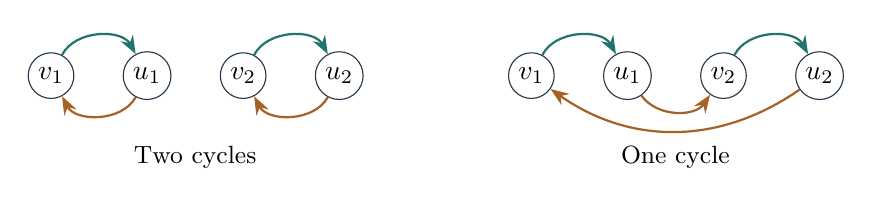
\begin{tikzpicture}[x=1cm,y=.65cm,>=Stealth,
 vert/.style={circle,draw=ink,fill=white,inner sep=2pt},
 leftpath/.style={sea,thick,->},rightpath/.style={ochre,thick,->}]
\foreach \i/\txt in {0/{v_1},1/{u_1},2/{v_2},3/{u_2}}{
 \node[vert] (v\i) at (\i*1.22,0) {\(\txt\)};
 \node[vert] (w\i) at (6.1+\i*1.22,0) {\(\txt\)};}
\foreach \n in {v,w}{
 \draw[leftpath] (\n0) to[bend left=62] (\n1);
 \draw[leftpath] (\n2) to[bend left=62] (\n3);}
\draw[rightpath] (v1) to[bend left=62] (v0);
\draw[rightpath] (v3) to[bend left=62] (v2);
\draw[rightpath] (w1) to[bend right=55] (w2);
\draw[rightpath] (w3) to[bend left=35] (w0);
\node[font=\small] at (1.83,-1.6) {Two cycles};
\node[font=\small] at (7.93,-1.6) {One cycle};
\end{tikzpicture}
\caption{The same left pairing (upper arcs) meets two different right pairings. For \(a=2\) the compatibility matrix has zeros on the diagonal and ones off the diagonal.}\label{fig:pairing}
\end{figure}

\subsection{How much rank is available?}

\begin{lemma}\label{lem:rank}
Over every field \(H_a\) contains a permutation submatrix of order \(2^{a-1}\). If the characteristic differs from two and \(a\) is nonzero in the field, then
\[
                     \rank H_a=\binom{2a-2}{a-1}.
\]
In particular, outside characteristic two \(\rank H_a\ge 4^a/a^{O(1)}\) for large \(a\).
\end{lemma}
\begin{proof}
Extend each permutation to fix \(a+1\), marking the extension with a hat, and put \(g=(a,a+1)\). Use rows \(\widehat\pi g^b\) and columns \(g^c\widehat\tau\) for \(b,c\in\bits\). If \(b=c\) the product fixes \(a+1\). Otherwise it inserts \(a+1\) in one old cycle and the test returns the old entry. This doubles the size of a permutation submatrix, starting with \(H_1=(1)\). It also embeds \(H_a\) in \(H_{a+1}\).

For the equality we may extend scalars to \(\olF\). On the subspace \(W=\{x\in\olF^a:\sum_i x_i=0\}\) the dot product is nondegenerate, since \(a\ne0\) in the field. A permutation \(\pi\) with cycle lengths \(d_1,\ldots,d_s\) has characteristic polynomial \(\prod_i(t^{d_i}-1)\). Removing the one trivial coordinate divides by \(t-1\). Evaluation at \(t=1\) therefore gives
\begin{equation}\label{eq:trace}
 \one_{\pi\ {\rm an}\ a\text{-cycle}}
   =a^{-1}\det(I-\pi|_W)
   =a^{-1}\sum_{j=0}^{a-1}(-1)^j\tr(\pi|_{\wedge^j W}).
\end{equation}
The last identity follows by expanding the determinant in principal minors.

We give the linear algebra showing that the group algebra acts on \(\bigoplus_j\wedge^j W\) as the full algebra \(\bigoplus_j\End(\wedge^j W)\). Write \(dA\) for the operator that applies \(A:W\to W\) to one factor at a time in a wedge and sums the results. For \(\alpha=e_i-e_j\), the transposition of \(i,j\) acts on \(W\) by \(I-\alpha\alpha^*\), where \(\alpha^*x=\angles{\alpha,x}\). Its action on the whole exterior algebra is \(I-d(\alpha\alpha^*)\), since two occurrences of \(\alpha\) in a wedge vanish. The image of the group algebra thus contains \(d(\alpha\alpha^*)\) for every root \(\alpha\). The roots \(\alpha_i=e_i-e_a\), \(i<a\), are a basis of \(W\). Taking their squares and those of \(\alpha_i-\alpha_j\) spans all symmetric operators, hence gives \(dA\) for every symmetric \(A\).

Choose an orthonormal basis of \(W\), using algebraic closedness and characteristic different from two. The commutator identity \([dA,dB]=d[A,B]\) follows by applying the operators to different wedge factors. From \(E_{ii}\) and \(E_{ij}+E_{ji}\) we obtain \(d(E_{ij}-E_{ji})\) by this identity, and then \(dE_{ij}\) by dividing by two. Here \(E_{ij}\) are the matrix units in the chosen basis. The operator \(dE_{ii}\) acts on a basis wedge by its indicator of containing index \(i\). Products of these operators and their complements therefore project onto \emph{individual} basis wedges across all degrees. Between two wedges of equal degree, successive one-index replacements by \(dE_{ij}\), with projections at the ends, realize any desired matrix unit up to sign. This proves the algebra assertion, including degrees zero and \(a-1\).

The matrix \(H_a\) represents the bilinear form \((x,y)\mapsto\varphi(xy)\) on the group algebra, where \(\varphi\) is the linear extension of \eqref{eq:trace}. On its image this is a sum of trace pairings on full matrix algebras with nonzero coefficients. Each trace pairing is nondegenerate, as can be seen on opposite matrix units. Pullback along a surjection preserves its rank. The rank is consequently \(\sum_j\binom{a-1}{j}^2=\binom{2a-2}{a-1}\). When the characteristic divides \(a\), apply the embedding from \(a-1\), which is then nonzero in the field. The central binomial estimate gives the final assertion.
\end{proof}

The characteristic-zero rank formula is also the bipartite connectivity formula of Raz and Spieker~\cite{rs,cln}. For our purposes set \(\rho=2\) in characteristic two and \(\rho=4\) otherwise. By Lemma~\ref{lem:rank}, \(\rank H_a\ge c\,\rho^a/(a+1)^C\) for absolute constants \(c,C>0\). Write \(R_m=\rank K_m\). Combining with \eqref{eq:patterncount} gives
\begin{equation}\label{eq:rankgrowth}
             R_m\ge (2+2\sqrt\rho)^m/m^{O(1)}\qquad(m\to\infty).
\end{equation}
Indeed, up to a polynomial factor the weighted sum is the constant coefficient of \((2+\sqrt\rho\,z+\sqrt\rho\,z^{-1})^m\), less \(2^m\) for \(a=0\). The coefficients are symmetric and largest at the center. To check the latter, a nonnegative symmetric unimodal sequence is a nonnegative sum of interval indicators centered at zero, and the convolution of two such indicators is symmetric unimodal. Here \(2\ge\sqrt\rho\). The center is at least the sum of all coefficients divided by \(2m+1\).

\subsection{Realizing the pairing test by a single tour}

We now construct the graph whose boundary has matrix \(K_m\). Every choice below on one side of a block is a function of that side's state only.

\paragraph{The prescribed paths.}
On each side lay down the paths of its pairing. On the first pair, in a fixed order, insert all vertices owned by that side for both arcs. Each of the other pairs is joined directly. On the left break the first arc \(x\to y\) of the first pair into \(x\to t_0\) and \(s_0\to y\) at two private vertices. When the two patterns agree, the joined paths give one spanning \(s_0\)-to-\(t_0\) path precisely when the unbroken pairings give one cycle. Any other cycle is confined to this block.

We must put \emph{all} choices in a single graph without leaving their unused private vertices uncovered. At each shared vertex \(v\), on each side, introduce two private vertices \(I_v,O_v\). Give the shared vertex the possible arcs \(I_v\to v\) and \(v\to O_v\). Route each prescribed local arc from the outgoing private vertex of its tail to the incoming private vertex of its head. Private terminals \(s_0,t_0\) use themselves at these connections. Call the private vertices used this way active. Prescribe a second, private path between two new terminals through \emph{all inactive} \(I_v,O_v\) on that side in fixed order. Use a direct connection if the list is empty. We will select exactly the private connections prescribed by this rule. Each inactive private vertex then has both degrees filled, and each active one forces its arc at \(v\). In particular, inconsistent patterns at a shared vertex cannot give a tour.

\paragraph{Selecting a connection.}
The table verifier guesses the state and computes a bit for each possible private connection indicating whether it was prescribed. Here is a directed version of the clause construction in Section~\ref{sec:transfer}. Represent a bit by a bidirected path, with forward traversal meaning true. In the clause order reserve a gap on the path for each literal. Put ordinary bidirected segments of length at least two between gaps and at either end. For a literal of clause \(C\), write its gap \(u,v\) in the direction that makes the literal true. Retain \(v\to u\) and replace \(u\to v\) by \(u\to C\to v\), where \(C\) is one vertex shared by the literals of the clause. Between successive bit paths put a connector accessible from either end of the first path and leading to either end of the next. Private start and end vertices make this entire verifier a segment. A private forward arc on each weighted bit path receives its weight.

In a spanning tour every ordinary segment has a consistent direction, since returning to the same neighbor at an interior vertex closes a two-cycle. At a gap, if one end requires the reverse arc \(v\to u\), that arc fills the corresponding need at both ends. Otherwise \(u\) needs its outgoing detour and \(v\) its incoming detour, forcing both arcs of the same literal. This prevents a tour from entering a clause through one occurrence and exiting through a different one. Each path has one direction and each clause is traversed exactly once. Conversely a satisfying assignment specifies the verifier traversal uniquely.

For a prospective private connection \(u\to v\) give its selection bit a private gap whose false-direction arc is \(x\to y\). Remove both prospective arcs. Introduce a fresh bidirected three-vertex path \(a,b,c\) and add
\[
                         u\to a,\quad c\to v,\quad x\to c,\quad a\to y .
\]
The reverse bit arc \(y\to x\) stays. The middle vertex \(b\) must use distinct neighbors, so a spanning tour traverses either \(u,a,b,c,v\) or \(x,c,b,a,y\), with a unique extension in either case. Contracting that path restores exactly one of the prospective arcs. In particular the bit traverses its false arc precisely when its private connection is unused. Surround the gap with ordinary segments just as for a clause occurrence.

Finally chain the verifier segments, the main segments \(s_0,t_0\), and all inactive-vertex path segments in one fixed cyclic order by their terminals. The main segment is attached at the earlier table, and each private segment at its own table. Order the attachments by table, so only a constant number of ends of this chain are ever live. For fixed local guesses, contracting all three-vertex paths leaves the prescribed block traversals and the verifier traversals. A tour exists precisely when every pattern agrees and each pairing closes one cycle before the break. When it exists it is unique. This proves the claimed compatibility matrix.

\paragraph{Using its rank.}
Put \(\ell=\lfloor\log_2 R_m\rfloor\). A nonsingular minor gives matrices \(U_0,V_0\) over the field with \(U_0K_m V_0=I_{2^\ell}\), by inverting the minor and restricting the identity. At each block end guess a physical state in addition to the logical word. If this is the left end, multiply by the corresponding entry of \(U_0\), and at the right end use \(V_0\). Each such entry can be emitted as a scalar weight of a true output when its word and state are guessed. Summing the guesses in the tour polynomial performs the matrix products, so the resulting logical block transmits equality. This construction uses a single graph even when some of the scalar entries are negative.

\paragraph{Width and degrees.}
Within one table all the blocks, relays, possible connections, and selection bits take \(O_m(T+d+1)\) vertices or bits before the serial lookup. Keep the endpoints of each bit path and one unfinished end during the clause sweep. Order the bit paths by first occurrence. The connectors between consecutive paths can then be installed when their endpoints are introduced, keeping the preceding path's endpoints until the next path starts, even if its clauses have already finished. This costs at most two extra vertices. Guards and clauses are generated at their occurrences. The width and size hypotheses of Lemma~\ref{lem:transfer} follow. Each shared vertex has indegree and outdegree at most two.

Here are details to bound the private degrees by three. A selector with one entry and \(b\) exits has a unique spanning path from its root to each chosen exit. To construct one, use a binary tree with the exits at its ordered leaves. Direct arcs from every internal node to its child roots. Give each child a representative leaf, and from that leaf add an arc to the other child root. A leaf represents itself. An internal subtree uses the rightmost leaf of its left child. Distinct internal subtrees determine distinct split gaps, so their chosen leaves are distinct. Each leaf supplies at most two crossing arcs and one external arc. Internal roots have at most two incoming and two outgoing arcs. A path ending in one child must first span the other, leave it through its representative, then span the desired child. Reentry into the first would revisit its root. Induction gives existence and uniqueness. Replace a high-degree private vertex by a reversed selector for its incoming arcs followed by a forward selector for its outgoing arcs. Their central arc is the only exit of the first and the only entry of the second. A spanning tour therefore traverses each selector just once. Keep old weights on the external arcs. At fixed \(m\) the affected private vertices have degree \(O_m(1)\), so the expansion preserves the layout. Equation~\eqref{eq:rankgrowth} and Lemma~\ref{lem:transfer} now give both directed lower bounds.

\subsection{Six states per vertex}

To match the lower bounds, first fix a root \(r\). A cycle cover is a selection of arcs using exactly one incoming and one outgoing arc at every vertex. After removing the arc out of \(r\), its remaining arcs form a tree oriented toward \(r\) precisely when the cover was a single tour. Work with basis vectors \(e_i\) for the vertices other than \(r\), and write \(e_r=0\). For each selected arc \(i\to j\) with \(i\ne r\), append \(e_i\) to one exterior product and \(e_i-e_j\) to a second. Multiply by the arc variable once, also for the selected arc out of \(r\).

For a complete cover, the coefficient in top degree of the two products together equals the determinant with columns \(e_i-e_j\) indexed by their tails. The first wedge supplies the sign for sorting the columns into tail order. If there is another cycle, its columns sum to zero. Otherwise order vertices by distance to the root. The matrix is triangular with diagonal one, so its determinant is one. Thus the weighted sum is exactly \(\hc(G)\).

On a path decomposition keep the current incoming and outgoing usage at each bag vertex. A basis wedge records which coordinates are occupied. In the first wedge this is already the outgoing usage. In the second, usage \(00\) implies unoccupied, since no incident arc has been taken. At usage \(11\) discard terms in which this coordinate is unoccupied, since no later column can fill it. Each mixed usage permits either occupancy. This gives \(1+1+2+2=6\) states per nonroot vertex. Forget only vertices with complete usage and, away from the root, complete occupancy. Order coordinates globally by forget time. Occupied forgotten coordinates make an initial segment in each wedge, so the sign for appending any coordinate is found by counting larger occupied live coordinates. A root has at most four states. Each arc thus costs polynomially many gates per entry and the bound is \(\OO(6^p)\) over any field.

\subsection{The smaller base in characteristic two}

We spell out the matching-basis update behind the characteristic-two algorithm of Cygan, Kratsch, and Nederlof~\cite{ckn}. It also explains why the same algorithm computes the formal polynomial with directed arcs and arbitrary characteristic-two weights.

Fix the outgoing arc \(u\to v\) of a root \(u\). We may assume there are at least two vertices and ignore loops. Delete that arc, introduce two new vertices \(s,t\), and force \(s\to v\) and \(u\to t\). A tour using the chosen arc corresponds to a spanning directed path from \(s\) to \(t\). Keep \(s,t,u,v\) available from the outset, adding at most four to the width. Initialize with the two forced arcs, and require all original vertices eventually to have one incoming and one outgoing arc. In the undirected view of a partial selection, its nontrivial components are paths, apart from premature cycles which we discard. Antiparallel arcs are separate edge choices, so a doubled undirected edge can be a two-cycle.

For a fixed vector of oriented degrees let \(E_1\) be the set of degree-one vertices, including \(s,t\), of even size \(b\ge2\). Each path joins a pair of \(E_1\). For a test matching \(M\) on \(E_1\), let \(T(M)\) sum the weights of the partial selections whose paths together with \(M\) close into one cycle. Unused live vertices have degree zero and are ignored by the test. Closed components in the partial selection give zero for every test, since \(s,t\) are endpoints. Once all original vertices are complete the only test is \(st\), so its value is the desired path sum.

Order the \(b\) endpoints. Divide them into a first singleton, successive pairs, and a last singleton. Use as \emph{chain tests} precisely the matchings with one edge between each two successive groups. Each pair group chooses which vertex receives the edge from the preceding group. There are \(2^{b/2-1}\) tests. We show how to process an arc in polynomial work per stored test.

\begin{lemma}\label{lem:localbasis}
On \(j=2,4,6\) sites every matching test is, in characteristic two, a linear combination of the chain tests in any prescribed order. This remains true with an arbitrary fixed collection of paths attached outside the sites, provided every site has one free end.
\end{lemma}
\begin{proof}
Index the rows and columns of a matrix \(H\) by perfect matchings of the sites. Set \(H[P,M]=1\) when their union is one cycle, counting a doubled edge as a cycle on two sites. We show that the columns for the chain tests span \(H\). On two sites there is just one matching. On four sites two different matchings close one cycle. Each row therefore contains two ones, so the three columns sum to zero in characteristic two. The two chain columns are independent, since on their own rows one reads \((0,1)\) and the other \((1,0)\).

On six sites two matchings close one cycle precisely when they are edge-disjoint. Consider the partitions of the edges of \(K_6\) into five perfect matchings. Every disjoint pair lies in exactly one such partition. Indeed, removing its six-cycle leaves two triangles joined by three disjoint edges. Each of the three remaining perfect matchings must use one joining edge. That edge determines the other two edges of its matching, one in each triangle.

A fixed perfect matching \(P\) has eight disjoint partners. Of the fifteen matchings, one is \(P\), and six others share one of its three edges. Each partition containing \(P\) accounts for four partners, so \(P\) belongs to two partitions. Counting incidences now gives \(15\cdot 2/5=6\) partitions in total. Let \(v_P\in\F^6\) indicate the two containing \(P\). In characteristic two,
\[
                         H[P,M]=\langle v_P,v_M\rangle .
\]
The dot product is one for a disjoint pair. Distinct matchings sharing an edge lie in no common partition, and for \(P=M\) the dot product is \(1+1=0\). Each \(v_P\) lies in the five-dimensional subspace of coordinate sum zero. The all-ones vector belongs to this subspace and annihilates it, so the restricted dot product has rank at most four. Hence \(\rank H\le4\).

There are four chain matchings on six sites. Two of them are edge-disjoint exactly when their choices at both middle pairs are opposite. An agreement gives the same edge at the first or last singleton, and two opposite choices leave all three edges different. Their four columns thus restrict to a permutation matrix on their four rows. They are independent and span \(H\). In all three sizes the restriction to the chain rows gives the coefficients of any desired test up to this permutation. For fixed outside paths, a separate cycle makes all tests zero. Otherwise the paths contract to a matching \(P\) on the free ends, so the same column identity applies to each completion and hence to every weighted sum.
\end{proof}

First, one may swap adjacent vertices in the order with constant work per new test. If the vertices belong to different groups, freeze all edges of the new test outside those two groups, leaving one exposed endpoint at each neighboring group that exists. At most six sites remain. The old tests extending the frozen edges restrict to exactly the chain tests on these sites, in their old order. Lemma~\ref{lem:localbasis} expresses the desired test using them. A swap within one group merely permutes the tests. Thus any reorder costs polynomial work per entry.

To introduce the arc \(i\to j\), either skip it, or take it when the two oriented degrees allow this. Move the affected endpoints to the end in the old and new orders, using adjacent swaps. For the take transition, pull a new test back across the arc. Place the undirected edge \(ij\) beside the new test and suppress vertices of degree two in this complementary collection. This leaves a matching on the old endpoints, unless it forms a closed complementary component, in which case the contribution is zero because the forced endpoints are elsewhere. More explicitly, two newly created endpoints are spliced out of their test edges, a single new endpoint is replaced by the endpoint that disappeared, and two disappearing endpoints are matched directly. This operation has exactly the one-cycle test of adding the arc to the partial paths.

The untouched endpoints form a common prefix in both orders and include \(s,t\). Take its longest odd-length initial part. In a chain test its internal edges leave one exposed vertex. Freeze those edges. The remaining local sites for the pulled-back test are this exposed vertex, at most one further untouched endpoint, and at most the two affected endpoints. The old chain tests with these frozen edges realize all chain tests on the remaining two or four sites. Lemma~\ref{lem:localbasis} again gives a constant-size update. Multiply the take transition by the arc variable and add it to the proper degree vector, restoring the original order. Introducing an unused vertex leaves every test unchanged. Forgetting an original vertex requires complete degrees, so it is absent from the endpoint list.

If \(b\) endpoints are mixed, the number of stored tests is at most \((\sqrt2)^b\). At each ordinary bag vertex the two neutral types \(00,11\) have factor one and each of the two mixed types has factor \(\sqrt2\). Summing over degree vectors gives \((2+2\sqrt2)^{p+O(1)}\) entries. Adjacent reorders, the choice of the root arc, and all bag operations give only polynomial factors. Multiply the final path sum by the deleted arc's variable and sum over the possible root arcs. Every tour occurs once. This finishes Theorem~\ref{thm:tours}.

\section{Pathwidth for directed and undirected tours}\label{sec:quant-transfer}

For directed cycles, \eqref{eq:rankgrowth} gives a nonsingular minor of order \(2^c\) on \(m\le c/\log_2 b+O(\log(2+c))\) sites, with \(b\) as in Theorem~\ref{thm:tours}. Index its rows and columns by \(c\) bits. The inverse minor on the left and the identity on the right realize logical equality by the construction of Section~\ref{sec:tours}. A physical state is stored by its minor index. For each candidate ordered pair of sites scan the list of indices to learn its selection bit, create its guard, and finish this bit before going on to the next pair. There are \(O(m^2)\) pairs. A scan emitting an entry of the inverse minor reads just \(2c\) address bits. The relays, live bit paths and private terminals therefore cost \(O(c)\) live vertices per wire, and the complete table has size \(2^{O(t)}\). The private degree-three selectors can be taken as combs with their leaves in incidence order. Each suffix has a leaf and the next suffix as children, with the latter's representative at its first leaf. Only constantly many additional vertices per live private vertex are needed at any cut in this order. Lemma~\ref{lem:quant-transfer} gives the two directed rows.

\subsection{Unoriented paths and matching connectivity}

For even \(j>0\) let \(M_j\) index perfect matchings of \(j\) labelled sites, with entry one when their union is one cycle (count the doubled edge at \(j=2\)). On \(m\) shared vertices a fragment specifies the left degrees \(0,1,2\) and pairs the degree-one sites by paths. The right degrees must be complementary. After permuting columns the compatibility matrix contains \(\binom mj2^{m-j}\) independent copies of \(M_j\) for each even \(j>0\). If \(\rank M_j\ge \rho^j/j^{O(1)}\), summing the even terms of the binomial expansion gives rank at least \((2+\rho)^m/m^{O(1)}\). Curticapean, Lindzey and Nederlof prove this with \(\rho=4\) in characteristic zero~\cite{cln}. In characteristic two the rank is \(2^{j/2-1}\)~\cite{ckn}. Every odd characteristic has at least the bipartite submatrix \(H_{j/2}\) from Lemma~\ref{lem:rank}, giving the lower estimate \(r_j\ge 2^j/j^{O(1)}\). Section~\ref{sec:modular} gives the exact growth in characteristic three.

Here is a graph implementing these blocks with one shared vertex per site. For each side prescribe the paths of its matching and insert all degree-two sites on the first path. Break one connection of the first left path at two private ends as in the directed construction. Give each site two private ports on each side. A selected incident path edge uses its own port. Join all unused ports on that side in fixed order into a private path with its own two ends. Retain the possible edge from each port to its shared site. An unused port has both incidences filled by the private path, and a used one must take its edge to the shared site.

For each possible private connection choose a fixed direction for its three-vertex guard, and compute its control bit in the verifier from Section~\ref{sec:tours}. Replace each verifier or guard vertex \(v\) by the undirected path \(v_{\rm in},v_{\rm mid},v_{\rm out}\). Attach every former directed incidence to its indicated port. Leave route vertices and route ends unsplit. The middle vertex forces traversal between the two ports of each split vertex. The selected incidences there give one former incoming and one former outgoing arc, and a directed two-cycle confined to split vertices would form a separate component. Thus the same clause and guard rules apply to the selected incidences. An active guard supplies one undirected connection to its route and an inactive guard occupies its prescribed gap in the verifier. Either traversal direction of a route gives the same selected edge set. Join the broken main paths, verifier paths and private unused-port paths in fixed cyclic order by their ends. A consistent choice yields exactly one spanning cycle edge set if the two matchings on each block close one cycle, and zero otherwise. Private vertices on the candidate connections also distinguish two sides prescribing the same pair. Inverting a minor and scanning its state numbers now proceeds exactly as for directed tours, with the same space and size estimates. The known path sweeps give the matching upper bases in characteristics zero and two~\cite{bckn,ckn}. Combining the same construction with Proposition~\ref{prop:mod3} gives the characteristic-three lower bound. This proves the undirected rows of Theorem~\ref{thm:additive}.

\section{Hamiltonian cycles across an edge cut}\label{sec:layouts}

On \(m\) boundary vertices the degree-one sites are paired. Each of the other sites has two possible degrees, giving \(R_2(m)\) as in Section~\ref{sec:quant-transfer}. For \(m\) crossing edges, a used edge has a single free end on each side and an unused edge has one state. The block for a fixed nonempty even set of used edges is \(M_j\), giving \(R_1(m)\). The following construction turns these edge ranks into unrestricted circuit lower bounds.

\subsection{Encoding a word on crossing edges}\label{sec:cut-blocks}

Use \(m\) disjoint edges, each joining a port at the earlier table to its counterpart at the later table. On either side choose a nonempty even subset of the ports and a matching of that subset. Prescribe one local connection per matched pair. Put the unused ports, in order, on the private path between two terminals. As in Section~\ref{sec:quant-transfer}, break the first pair on the earlier side at two further terminals, and visit the broken main paths, private paths and verifiers in their fixed cyclic order. Each prospective connection has its own guarded route. A used port has one prescribed local incidence and requires the crossing edge. An unused port already has two local incidences. Thus inconsistent subsets give zero. For consistent subsets a spanning tour exists precisely when the two matchings close one cycle before the break. Its selected edge set is unique for those guesses. This gives the direct sum defining \(R_1(m)\).

For directed graphs, distinguish the two directions on a crossing adjacency. A used set now has \(a\) arcs each way. Each side pairs the two sets by a bijection, using directed local paths, and the same break is taken on the earlier side. Unused ports are again put on a private directed path. A used port requires the unique crossing direction complementary to its local incidence. The compatibility test on fixed direction sets is the one-cycle permutation matrix \(H_a\) of Lemma~\ref{lem:rank}. Write \(h_a=\rank_\F H_a\) and let \(\sigma=2\) in characteristic two and \(4\) otherwise. Then \(h_a\ge\sigma^a/a^{O(1)}\). In characteristic two equality \(h_a=2^{a-1}\) also follows by embedding \(H_a\) in \(M_{2a}\) and using the matching rank~\cite{ckn}.

For underlying cutwidth allow both directions on each of \(m\) crossing adjacencies. For arc cutwidth take \(m\) even and prescribe just one direction per adjacency, half in each direction. The respective block ranks are
\[
 \sum_{a\ge1}\binom m{2a}\binom{2a}a h_a
       \ \ge\ \frac{(1+2\sqrt{\sigma})^m}{m^{O(1)}},\qquad
 \sum_{a\ge1}\binom{m/2}a^2 h_a
       \ \ge\ \frac{(1+\sqrt{\sigma})^m}{m^{O(1)}} .
\]
The first inequality uses the central binomial estimate and the even binomial sum. For the second, apply Cauchy--Schwarz to \(\binom{m/2}a(\sqrt{\sigma})^a\) over \(a\ge1\). These calculations count dimensions over the integers in every characteristic.

\paragraph{Cost in minimum cutwidth.}
Suppose a block has rank at least \(b^m/m^{O(1)}\). Invert a nonsingular minor on the earlier side, as in Section~\ref{sec:tours}, to realize equality on \(l_m\ge m\log_2 b-O(\log m)\) bits. Use the source of Proposition~\ref{prop:quant-source} and take \(m\) even with \(m=\Theta(\sqrt t)\). Split each word of \(c\) bits into \(\lceil c/l_m\rceil\) blocks, pinning the unused logical bits of its final block. Since at most \(w+1\) words cross a table boundary, its physical edge count is at most
\[
 \frac{D}{\log_2 b}
       +O\!\left(t+\frac{D\log m}{m}+wm\right)
       =\frac{D}{\log_2 b}+O(t).
\]
Here \(D=wt\) and \(t=\Theta(w^3(\log(2w))^{3/2})\). The estimate counts an antiparallel pair once only in the underlying-edge convention.

Within a table, process one block at a time. Its \(O(m^2)\) candidate port connections and private routing edges cost \(O(t)\) crossing edges even if charged simultaneously. Generate each guard and its selection bit at its serial lookup. Keep the table's logical bits, the current physical index and the bounded-degree bit paths of the verifier, with \(O(t)\) unfinished ends altogether as in Section~\ref{sec:quant-transfer}. Only the current block needs its private routing graph. The incident blocks have \(O(t)\) exterior ports in total, and the fixed chain connecting the terminal pairs contributes \(O(1)\) more edges between blocks. These bounds count arcs individually inside a directed table if required. The size is \(2^{O(t)}\). Thus the minimum cutwidth \(k\) satisfies \(k\log_2 b\le D+O(t)\), and specializing the output gives \(\log_2 s_\F\ge D-O(t)\). The pathwidth upper bounds and \(\pw\le k\) give \(k=\Omega(D)\), so \(t=\Theta(E(k))\).

For undirected tours this proves the additive estimate at \(b=1+u\) under the quantitative hypothesis of Proposition~\ref{prop:rank-rate}. The vertex construction gives the corresponding estimate at \(2+u\). Taking a sufficiently large fixed minor excludes every base strictly less than \(1+\rho_\F\) or \(2+\rho_\F\), respectively, even after any fixed polynomial factor in \(n\). An additive estimate at the limiting base from this construction requires control of how fast the rank grows. In characteristic zero, two and three the bounds in Section~\ref{sec:quant-transfer} give this control.

\subsection{Scalar updates at an edge cut}\label{sec:cut-upper}

First consider a directed cycle cover. Fix a root, leave its cycle unmarked, and sum over markings of the other cycles with a factor \(-1\) per marked cycle. A cover with any other cycle cancels. One spanning cycle contributes its edge monomial once. For graph order at least three, every cover containing a loop or a two-cycle contributes zero after summing over markings, so we may discard those covers. At an underlying edge the possibilities are absence or either direction with either mark. When treating arcs separately there are just three possibilities per arc.

To compute the signs, let \(S\) be the set of marked vertices and let \(\pi_S\) send each to its successor. The desired sign is \((-1)^{|S|}\operatorname{sgn}(\pi_S)\). An inversion of two marked arcs requires their closed endpoint intervals in the vertex order to overlap. Charge the inversion at their first common position. At that point both states are known, including the case where one interval ends as the other begins. At a vertex choose its incoming and outgoing arc and their common mark, imposing an unmarked root. All other incident arcs are absent. Multiply by the new arc weights on their first occurrence, the vertex sign and the signs of the inversions charged there. There are polynomially many choices per incoming table entry, even at a vertex of large degree. This proves the \(n^{O(1)}5^k\) and \(n^{O(1)}3^k\) bounds in the two directed conventions. For an undirected graph in characteristic zero, allow both orientations, identify their weights, and divide the resulting polynomial by two.

For the smaller modular bases, an edge cut stores one inactive state per unused edge and one open strand per used edge. In an underlying directed cut also store the direction of each used edge. To use the spanning-path tests without dividing by two, fix a root and its unordered pair of neighbors in an undirected tour, delete the root, and leave one external end at each prescribed neighbor. Sum over the pairs with both incident edge weights. In a directed tour fix the ordered predecessor and successor instead. The two external ends take \(O(1)\) additional positions. At the current vertex enumerate its two selected incidences with the required directions, counting an external end as an incidence. For a given choice all other incident edges are unused. Two old open ends are joined, an old end is transferred to a new one, or a pair of new ends is created. Weights are charged once. Only these two positions and the unchanged open ends need be present during an update, even if the old and new cuts together contain many incident edges.

In characteristic two, the chain tests and adjacent swaps of Section~\ref{sec:tours} perform each such change with polynomial work per entry. On \(j\) open ends they use \(O((\sqrt2)^j)\) entries including the external ends. Summing over their positions gives the upper base \(1+\sqrt2\) for undirected or fixed-direction crossings, and \(1+2\sqrt2\) when each used edge can have either orientation. Bojikian, Chekan and Kratsch obtain the same undirected edge base for randomized Hamiltonicity decision and a conditional lower bound for that decision problem~\cite{bck-cutwidth}. Here the updates compute the full edge-weight polynomial over a field of characteristic two.

In characteristic three, use the form, three retained types and tensor-tree update of Proposition~\ref{prop:mod3}. On \(j\) open strands and a bounded number of external ends the retained space has dimension \(O(\rho_\F^j)\). Unused edges fix the unit type. The two affected leaves can be placed at the end of the common order using adjacent swaps, each an equivariant map on two leaves. Only their ancestors in the balanced tree change labels, at polynomial cost per coordinate as in that proposition. Joining, transferring or creating the selected pair has the same cost. Summing over subsets now gives \(n^{O(1)}(1+\rho_\F)^k\). The signed even and odd strand calculation of Section~\ref{sec:modular} works on the same edge cuts for every fixed prime \(\ell\ge5\). A used edge carries two even trivial types and the odd natural module. Its retained dimension grows at most as \(u_\ell^j\) on \(j\) sites, with \(u_\ell=2+2\cos(\pi/\ell)\). Thus \(1+u_\ell\) is an upper cutwidth base and \(2+u_\ell\) is an upper pathwidth base. Pinning the distinguished strand to an even color gives a factorization of \(M_j\) through the same retained space, so \(\rho_{\mathbb F_\ell}\le u_\ell<4\). A dimension bound for a new field also needs a way to implement its local updates in few scalar gates. This completes the upper bounds of Theorem~\ref{thm:layouts}.

\section{Linear sweeps and scalar updates}\label{sec:frontiers}

A coefficient matrix at a cut has rows indexed by monomials in the past input variables and columns by monomials in the future variables. If all dependence across the cut passes through \(d\) scalar entries and the output is linear in them, the matrix is a sum of \(d\) rank-one matrices. This gives a direct lower bound for the number of stored entries.

Join every vertex of a \(k\)-clique to every vertex of a disjoint \(k\)-vertex path. Keeping the clique live permits its edges to be processed first. The resulting bags and the clique of size \(k+2\) give \(p=k+1\). For directed tours use both arc orientations. Every prescribed fingerprint with an open path is realizable on the clique, by inserting all degree-two sites in the first path. On the other side subdivide each connection except the last with one private path vertex, and subdivide the last with the entire remaining consecutive suffix. There are at most \(k-1\) connections. Selected monomials determine their fingerprints, so the coefficient matrix contains the compatibility blocks of Section~\ref{sec:quant-transfer}.

\subsection{Scalar gate counts for Hamiltonian cycles}

In the directed determinant sweep of Section~\ref{sec:tours}, let \(i,o,y\) indicate a live nonroot site's incoming usage, outgoing usage and second-wedge occupancy. The total charges \(o-i\) and \(y-o\) are fixed once the root data are known, since each arc has one incidence of each direction, each selected nonroot tail supplies one factor to each wedge, and a forgotten nonroot site is complete. The states of degree zero and two have charge zero. After an invertible integer change of charge coordinates the four degree-one states contribute \(\pm e_1,\pm e_2\). For \(m\) fixed degree-one sites their two diagonal-coordinate sums are sums of independent fair signs, so any prescribed endpoint occupies at most \(O(4^m/(m+1))\) entries. Summing over their locations under weights \(\binom km4^m2^{k-m}\) yields \(O(6^k/(k+1))\) entries, since \(m\) is binomial with mean \(2k/3\). Each arc has constantly many transitions per entry with wedge signs determined by the indices. The exact gate bound is \(O(n6^p/(p+1))\).

For an undirected characteristic-zero sweep, use the signed strand calculation of Section~\ref{sec:modular}. Split a root into two ends of degree one and allow each former incident edge to attach to either end, retaining its weight. Fix opposite isotropic even colors at the external ends with pairing one. A path joining them contributes one, each extra cycle contributes zero, and each spanning tour has two choices of root assignment. Divide by two at the end. Using both copies of a single old edge would confine the joining path to one neighbor and leave extra cycles when \(N>2\). Small graphs are handled directly. Thus the root costs only a constant number of slots and a constant factor in events.

In an isotropic basis of the even plane record its two colors explicitly with charges \(+1,-1\). On the odd plane use the standard two-dimensional \(\mathrm{SL}_2\) representation. For a fixed collection of \(i\) even-strand and \(j\) odd-strand sites, the charge condition allows \(O(2^i/\sqrt{i+1})\) even assignments. The odd tensor is invariant. For even \(j\) its invariant space has dimension \(\binom j{j/2}/(j/2+1)\), and for odd \(j\) it is zero. Under the characteristic-zero rule \(V_a\otimes V_1=V_{a-1}\oplus V_{a+1}\), with \(V_a=\operatorname{Sym}^a K^2\) and \(V_{-1}=0\), paths of labels starting and ending at zero count the Catalan number. For \(m=i+j\) given open sites, the binomial sum over \(i,j\) has \(O(4^m/(m+1)^2)\) coordinates, since both are linear in \(m\) except for exponentially small tails. Counting the neutral sites gives \(O(6^k/(k+1)^2)\) in a bag.

Keep the odd tensor in a balanced binary coupling tree on the slots~\cite{singh-vidal}. Each leaf carries \(V_0\) or \(V_1\), and coupling \(V_a,V_b\) gives one copy of each \(V_c\) with \(c=|a-b|,|a-b|+2,\ldots,a+b\). For any physical edge move one endpoint leaf towards the other by tree rotations. Each rotation involves that individual leaf. Once the four incident branch labels are known, coupling with its label zero or one permits at most two intermediate labels. The basis change is therefore a matrix of order at most two per fixed block. Interchanging branches contributes a scalar on a multiplicity-one component and the prescribed odd sign. After \(O(\log(p+2))\) rotations the two slots are siblings. Apply the local cup, cap, transfer or skip in a constant-size block and undo the rotations. Slot degrees are fixed throughout every change of basis. The intertwiners can be chosen over the rationals, and the even isotropic basis needs at most a constant-degree extension. The exact gate count is
\[
                  O\bigl(n6^p\log(p+2)/(p+1)^2\bigr).
\]

A bipartite past or future gives an additional saving for either tour sweep. The selected degrees \(d_v=0,1,2\) obey a prescribed signed sum \(\sum_B s_v d_v\), since private vertices have selected degree two. Use \(2-d_v\) on the future side. Open sites have \(d_v=1\), and on the neutral set \(U\) each \(d_v-1\) is a sign. For fixed \(U\), one balance retains at most a central-binomial fraction \(O(1/\sqrt{|U|+1})\) of its choices. With two bicolorings agreeing on \(A\) the fraction is \(O(1/\sqrt{(|U\cap A|+1)(|U\setminus A|+1)})\). Relative to the weights above, each site is neutral independently with probability \(1/3\). Binomial concentration gives an additional factor \(O(1/\sqrt{p+1})\) in the one-side gate bounds, or \(O_\delta(1/(p+1))\) if the agreement and disagreement groups have size at least \(\delta k\) at every large cut. Conditioning on the root states costs only a constant. The projections are valid on each contributing degree pattern, including configurations that cancel at the end. The undirected basis rotations preserve each ordinary slot's degree. Thus on every bipartite host the directed bound is \(O(n6^p/(p+1)^{3/2})\) and the undirected bound is \(O(n6^p\log(p+2)/(p+1)^{5/2})\) in characteristic zero.

\paragraph{Savings on small hosts.} Write \(N=|V|\) and let \(g\ge0\). For either tour polynomial, subset dynamic programming for paths from a fixed root costs \(2^N\operatorname{poly}(N)\) gates. For undirected cycles, prescribe the smaller of the two root neighbors as the first and the larger as the last and sum over neighbor pairs. This counts each cycle once in every characteristic. Hence \(N\le p\log_2 b-g\) suffices at any of the stated tour bases \(b\).

\subsection{Sums of independently ordered sweeps and binary contractions}\label{sec:orders}

The preceding fixed-cut examples allow a program to choose a better variable order. The following construction permits each summand to choose its own order, or even its own binary tree on the input variables. A tensor on one such tree has \emph{width} \(w\) if its coefficient matrix at every tree-edge cut has rank at most \(w\). Binary contractions with bond dimensions at most \(w\) have this property. A read-once linear sweep of width \(w\) gives the property on the caterpillar for its order, taking the coefficient of degree zero or one at a variable leaf. The graph parameter of the following theorem is pathwidth.

\begin{theorem}\label{thm:orders}
For each row of Theorem~\ref{thm:additive}, each sufficiently large even \(k\), and \(h\ge1\), there is a graph of pathwidth \(p=k+O(1)\) and size \(\operatorname{poly}(k,h)\) such that any sum of \(h\) tensors with independently chosen binary variable trees must have
\[
                       \sum_{i=1}^h w_i\ge 2^L/k^{O(1)} .
\]
For each fixed \(C\) and \(h=2^{o(\sqrt k)}\), this excludes total width \(n^C2^{L-\sqrt p}\) on all such graphs.
\end{theorem}

\paragraph{The graphs used in the rank test.}
On \(k\) shared sites make \(M\) copies of a graph fragment, each with \(O(k^2)\) private vertices and its own marked variables. We require two simultaneous operations. Two active fragments give a matrix of rank \(R\ge 2^L/k^{O(1)}\) on their respective sets of marks. Every other fragment can independently give a factor of rank two on any two of its marked variables. It can also be set to a nonzero scalar. The following construction realizes both operations for tours.

For tours split one distinguished site into \(s,t\). A fixed chain from \(t\) to \(s\) passes through all fragment verifiers. In an active fragment there is a selectable route for every pair of ordinary sites and the two new ends, in both ordered directions in the directed case. A selected route is tagged once. We give its physical implementation so that the same tags also work when the fragment is neutral. For candidate \(u,v\) use bidirected private triples \(d,w,x\), \(y,h',e\), and \(a,b,c\), marking \(w\to d\). In active mode use the links
\[
             x\to c,\quad a\to y,\quad y\to x,\quad u\to a,\quad c\to v .
\]
A traversal \(d\) to \(e\) uses the middle triple from \(c\) to \(a\). A traversal \(e\) to \(d\) takes \(y\to x\), uses the marked arc and forces the route \(u,a,b,c,v\). The middle vertices of the triples require distinct neighbors in a spanning tour. Private connectors between consecutive candidates give each bit either traversal direction. In neutral mode remove the exterior arcs and \(y\to x\), and retain both directions on \(x,c\) and \(a,y\). Connect the resulting bidirected nine-vertex paths end to end through the same connectors. The fragment's entrance can enter either outer end and either end can lead to its exit. It now has just two spanning traversals, of total weight \(1+\prod z_i\). Start with the union of these two possible edge sets, so selecting a mode deletes only unmarked arcs.

For undirected tours split each private vertex into its forced in--middle--out path as in Section~\ref{sec:quant-transfer}. A selected route can then be traversed in either direction. The two neutral traversals have different selected marked edges. Use two active fragments and keep all other fragments neutral. Choosing the tags on each active fragment prescribes all the selected paths. Realize any fingerprint with the distinguished site mixed by inserting degree-two sites in its first path. Replace its distinguished occurrence on one side by \(s\) and on the other by \(t\), with \(s\) the path start in the directed case. Contracting the fixed verifier chain restores that site. The two selected monomials give one spanning cycle precisely for compatible fingerprints, and distinct fingerprints have different monomials. Requiring one distinguished open site retains at least a \(1/k\) fraction of every nonempty compatible-degree family (at least \(a/k\) with \(a\) mixed sites of prescribed direction). Thus \(R\ge 2^L/k^{O(1)}\) by the ranks already proved. Neutral fragments supply independent factors at the same time. There are only constantly many extra live ends, and one active fragment contains a clique minor on the ordinary sites. This proves \(p=k+O(1)\) for the tour hosts as well.

These fragments have the two properties used in the independent-fragments lemma of \href{sharp-pathwidth-bases.pdf}{\emph{Sharp Width Bounds for Counting Polynomials}}, in the appendix on independently ordered sweeps. That argument selects one cut per tree, keeps two active fragments unsplit on opposite sides, and uses the neutral fragments to obtain \(\sum_i w_i\ge2^{\lfloor\log_2 R\rfloor}\). Applying it here proves Theorem~\ref{thm:orders}.

\section{Four matching indices in Euclidean space}
At two sites \(x,y\) the Euclidean tensor price~\cite{euclid} of \(M_j\) is \(\|x-y\|\log_2 r_j\), since local linear maps convert the matrix to an equality wire of dimension \(r_j\) and back. The substitution in Section~\ref{sec:rank-rate} also lets us retain the row and column of each block as separate indices. Two blocks of size \(b\) then give two independent \(q\)-dimensional wires, \(q=r_b\), inside the restricted matrix on \(2b-2\) vertices.

Place these two wires on the diagonals of a unit square. To express \(t\) copies, let each summand start from \(a\) copies of the two horizontal wires and \(t-a\) copies of the two vertical wires, all of dimension \(q\), with its own choice of \(a\) and arbitrary local linear maps. The target costs \(2\sqrt2\,t\log_2 q\), each supply costs \(2t\log_2 q\), and the square has normalized mean width two. The sum inequality gives \(L\ge q^{(\sqrt2-1)t}\) summands even with cancellation. This bounds the cost of this four-site implementation. A stronger rank bound would require converting an arbitrary two-site rank factorization into a sufficiently cheap four-site implementation.

\bibliographystyle{../linkedtitles}
\bibliography{../references}
\end{document}
